

 
\documentclass[11pt,a4paper]{article}
\usepackage[utf8]{inputenc}		% LaTeX, comprend les accents !
\usepackage[T1]{fontenc}
\usepackage{natbib}	
%\usepackage[square,sort&compress,sectionbib]{natbib}		% Doit être chargé avant babel      
\usepackage[frenchb,english]{babel}
\usepackage{lmodern}
\usepackage{a4wide}
\usepackage[capposition=top]{floatrow}
\usepackage{verbatim}
\usepackage{float}
\usepackage{placeins}
\usepackage{flafter}
\usepackage{longtable}
\usepackage{import}
\usepackage{pdflscape}
\usepackage{rotating}
\usepackage{hhline}
\usepackage{multirow}
\usepackage{booktabs}
\usepackage[pdftex,pdfborder={0 0 0},colorlinks=true,linkcolor=blue,urlcolor=blue,citecolor=blue,bookmarksopen=true]{hyperref}
\usepackage{eurosym}
%\usepackage{breakcites}
\usepackage[autostyle]{csquotes}
%\usepackage{datetime}
\usepackage{natbib}
\usepackage{setspace}
\usepackage{lscape}
\usepackage[usenames]{color}
\usepackage{indentfirst}
\usepackage{url}
\usepackage{enumitem}
\usepackage{multirow}
\usepackage{subcaption}
\usepackage[justification=centering]{caption}
\bibliographystyle{agsm}

\usepackage{array}


\selectlanguage{frenchb}

\newcommand{\isEmbedded}{true}



\begin{document}

\title{Point d'étape CNRACL}


\maketitle

\section{Complétion des durées initiales}

\subsubsection*{Résumé:}

\begin{itemize}[leftmargin=1cm ,parsep=0cm,itemsep=0cm,topsep=0cm] 
\item \textbf{Objectif:} Trouver une durée initiale passée dans le grade pour l'ensemble des individus (population: dans le corps AT en 2011). 
\item \textbf{Approche:} Utiliser les trajectoires d'indices pour retrouver la date du changement de grade en localisant la sortie de grille en prenant en compte (i) les potentiels chevauchement de grilles et (ii) les délais de mise en oeuvre des grilles. 
\item  \textbf{Résultat:} Graphes sur la survie dans l'état et écarts entre duree min et max à venir. \\ A la fin de la procédure de complétion (en 2007 pour l'instant, date de création du grade des AT), les individus peuvent être dans 3 statuts différents: (i) Identifié comme étant sorti du grade entre 2007 et 2010, (ii) Identifiés comme n'étant pas sortis du grade entre 2007 et 2010 et (iii) Dans une situation d'ambiguïté dû à un chevauchement qui a toujours cours en 2007. Nous considérons les observations pour les individus (ii) et (iii) comme \textbf{censurés à gauche}. 

\begin{table}[ht]
\centering
\begingroup\footnotesize
\begin{tabular}{lccccc}
  \hline
 & Tous & TTH1 & TTH2 & TTH3 & TTH4 \\ 
 Nb d'individus & 187102.00 & 119089.00 & 30286.00 & 27982.00 & 9745.00 \\ 
   \hline
Nb non censurés & 105058.00 & 55865.00 & 22081.00 & 19324.00 & 7788.00 \\ 
  Prop non censurés & 0.56 & 0.47 & 0.73 & 0.69 & 0.80 \\ 
   \hline
Nb d'ind censurés & 82044.00 & 63224.00 & 8205.00 & 8658.00 & 1957.00 \\ 
  Prop censurés & 0.44 & 0.53 & 0.27 & 0.31 & 0.20 \\ 
   \hline
\end{tabular}
\endgroup
\end{table}

 
\end{itemize}



\subsubsection*{Améliorations futures:}

\begin{itemize}[leftmargin=1cm ,parsep=0cm,itemsep=0cm,topsep=0cm] 
\item Limiter l'écart entre dureemin et dureemax en neutralisant les chevauchements impossibles. 
\item Limiter l'importance de la censure à gauche: 
\begin{enumerate}[leftmargin=1cm ,parsep=0cm,itemsep=0cm,topsep=0cm] 
\item Hypothèses fortes avant 2007 (ex: an aff = entrée dans le grade)
\item Attente des grilles du corps avant 2006 pour prolonger la complétion. 
\end{enumerate}

 \item Pas trimestriel? 
\end{itemize}


\section{Estimations}


\subsection*{Sélection de l'échantillon:}

METTRE ICI le tableau des filtres


\subsection*{Cadre empirique}

Modèle de durée avec: 
\begin{enumerate}[leftmargin=1cm ,parsep=0cm,itemsep=0cm,topsep=0cm] 
\item Censure à droite (certains spells pas finis en 2015). 
\item Troncature à gauche: en prenant les spells observés en 2011 et commencés avant on sélectionne des spells relativement long. Par exemple un spell commencé en 2007 et fini en 2010 n'est pas observé. 
\item Censure à gauche: on n'observe pas la date de début d'entrée pour certains individus (cf. complétion). 
\end{enumerate}

Pour l'instant on ne gère pas la troncature ni la censure à gauche. 

Question: censure à droite endogène (informative)? 


On se concentre pour l'instant sur un seul grade, avec une censure à gauche et à droite limitée (Grade TTH3). 




\subsection*{Kaplan-Meyer}

\begin{figure}[H] 
  \caption{Estimation des survies par grade (Kaplan-Meyer)}
  \label{censure} 
    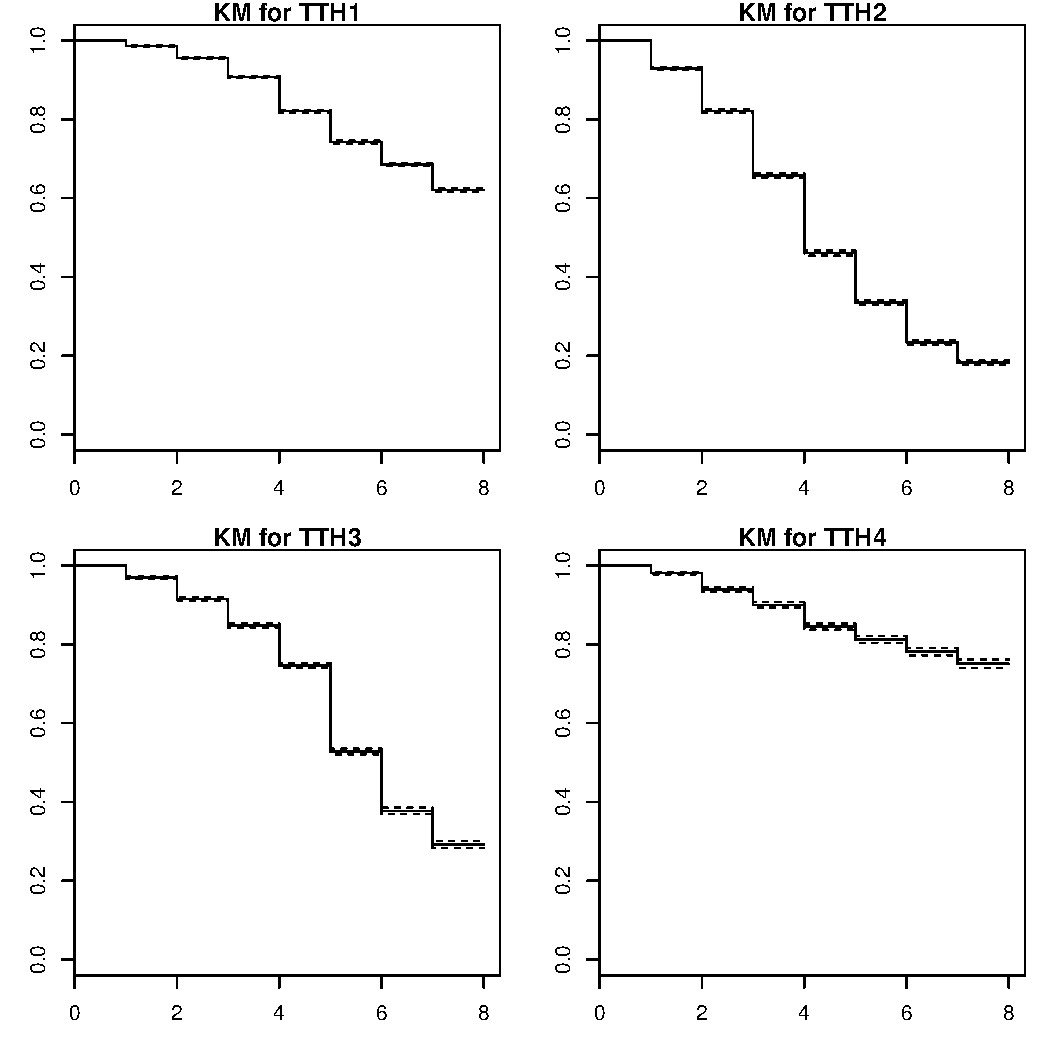
\includegraphics[scale = 0.75]{KM.pdf} 
\end{figure}



\subsection*{Estimation paramétrique}

Test de modèle de durée classique avec les spécifications usuelles du de la fonction de hazard. 
\begin{itemize}[leftmargin=1cm ,parsep=0cm,itemsep=0cm,topsep=0cm] 
\item Exponentiel (risque constant)
\item Weibull (risque variable)
\end{itemize} 

On se concentre sur la population des TTH3, pour laquelle la censure à droite et à gauche est limitée. Le modèle Weibull semble donner des résultats satisfaisants. Toutefois, la forme est fortement déterminé par la spécificité institutionnelle du grade. 


\begin{figure}[H] 
  \caption{Comparaison des estimations paramétriques simples}
    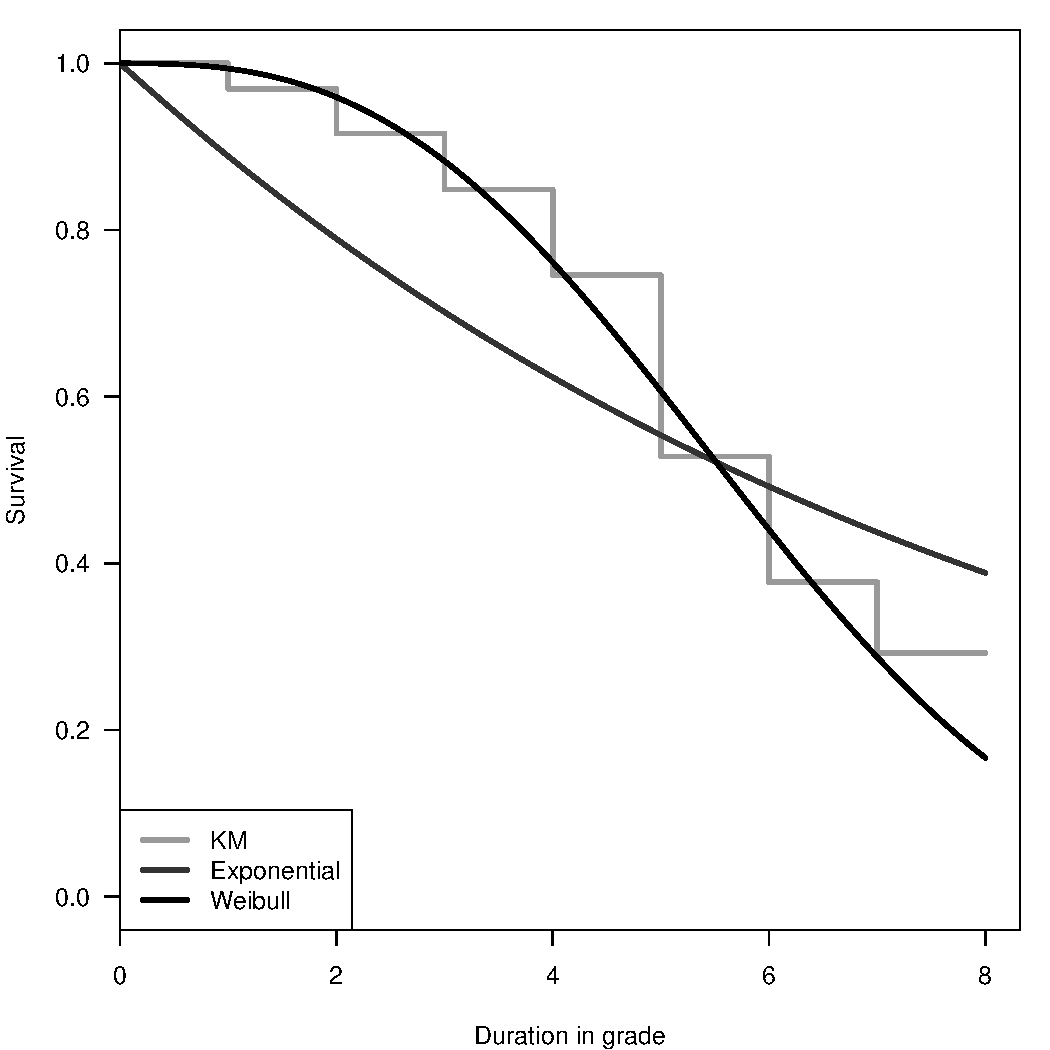
\includegraphics[scale = 0.6]{comp.pdf} 
\end{figure}




\subsection*{Utiliser les variables institutionnelles:}

KM + note précédente: impact des conditions de grade et d'échelon sur la probabilité de sortie du grade. Intégrer dans les variables explicatives les conditions. 
A ce stade nous utilisons uniquement la condition de durée dans le grade, qui est la plus simple à calculer. 

\begin{itemize}[leftmargin=1cm ,parsep=0cm,itemsep=0cm,topsep=0cm] 
\item Même cadre que Card/Chetty/Weber sur l'impact de la durée d'indemnisation sur la proba de sortir du chômage. 
\item Prise en compte de variables qui varient avec le temps. 
\item Problème à ce stade: variation identificatrice vient de différents individus qui atteignent les seuils à différentes durée dans l'état. Notre cadre avec un seul grade et une seule condition de grade ne convient pas. 
\item[] $\Rightarrow$ incorporer les échelons et plusieurs grades en même temps. 
\end{itemize}

\subsection*{Suite}

\begin{itemize}[leftmargin=1cm ,parsep=0cm,itemsep=0cm,topsep=0cm] 
\item Avancer sur le time-varying (plusieurs grades, conditions d'échelon). 
\item Aborder le multi-state? Time-varying + multi-state: pas de packages. 
\item Arriver rapidement à la simulation. 
\item Problème de la censure: besoin d'observer des durées plus longues (indispensable en simulation). 
\end{itemize}


\section{Divers}

\subsubsection*{Données}

\begin{itemize}[leftmargin=1cm ,parsep=0cm,itemsep=0cm,topsep=0cm] 
\item Toujours des nouveaux problèmes: qualité de l'information se dégrade fortement (et de manière discontinue au cours du temps). 
\item Lien avec la CDC pour qu'ils fassent le job. 
\item Question des variables utilisées pour l'estimation et leur présence en projection. 
\end{itemize}

\subsubsection*{Policy variables}

Quelles sont les variables que l'on souhaite pouvoir modifier pour simuler des changements de grilles? Envisage-t-on des comportements endogènes ou exogènes? Seuls les déterminants  intégrés à la modélisation auront un impact direct sur les comportements. 



\subsubsection*{Turin}

\begin{itemize}[leftmargin=1cm ,parsep=0cm,itemsep=0cm,topsep=0cm] 
\item Billet/hôtel
\item Autre? Parler de bigdata?
\end{itemize}



\end{document}







